\begin{figure*}[htbp]
\vspace{-\baselineskip}
    \centering
    \begin{tabular}{m{38mm} m{38mm} m{40mm} m{5mm}}
        \begin{minipage}[b]{40mm}
            \centering
            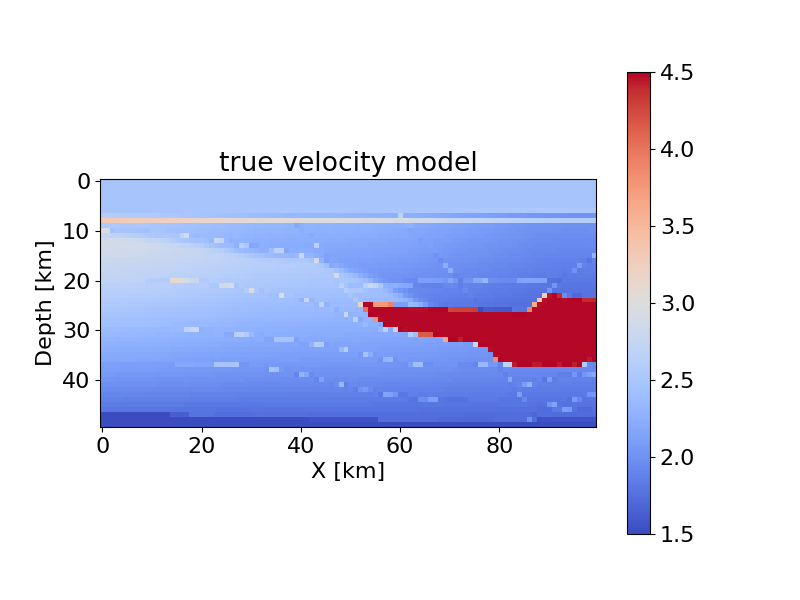
\includegraphics[width=40mm]{public/true}
            \vspace{-7mm}
            \caption*{\raisebox{2mm}{Background truth}}
        \end{minipage} &
        \begin{minipage}[b]{40mm}
            \centering
            
\includegraphics[width=40mm]{public/initial}
            \vspace{-7mm}
            \caption*{\raisebox{2mm}{Initial model}}
        \end{minipage} &
        \begin{minipage}[b]{40mm}
            \centering
            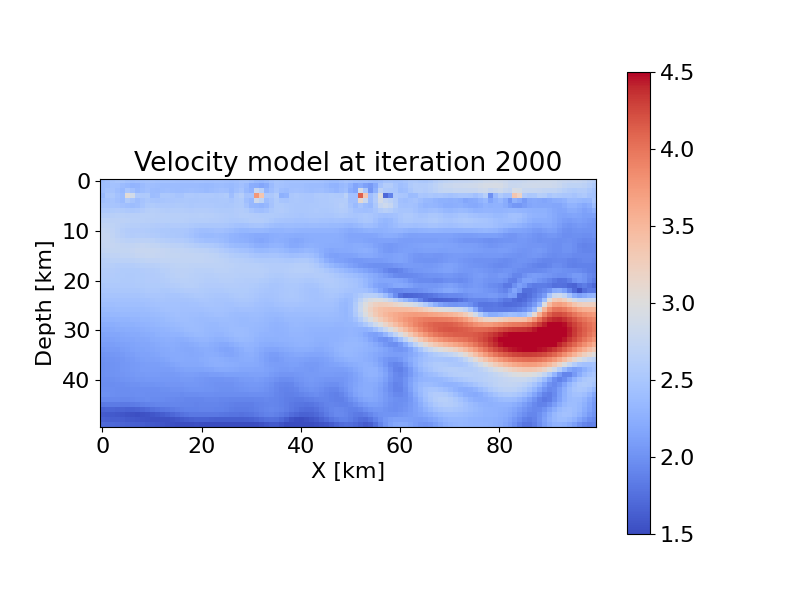
\includegraphics[width=40mm]{public/gradient}
            \vspace{-7mm}
            \caption*{\raisebox{2mm}{Standard FWI}}
        \end{minipage} &
        \multirow[t]{2}{*}{\raisebox{-34mm}{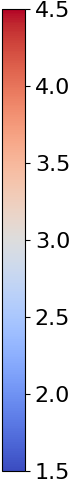
\includegraphics[height=50mm]{public/color-bar}}} \\
        \begin{minipage}[b]{40mm}
            \centering
            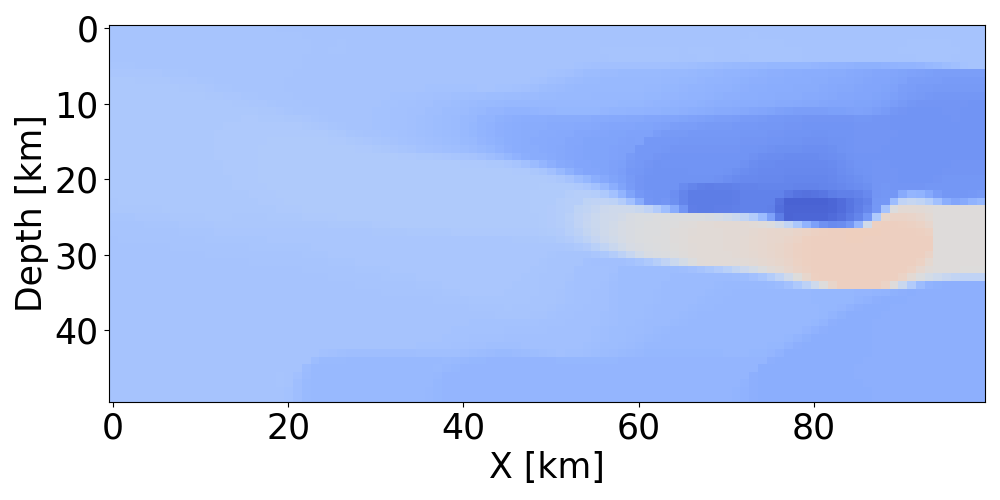
\includegraphics[width=40mm]{public/alpha_150}
            \vspace{-8mm}
            \caption*{Proposed Method, $\alpha$=150}
        \end{minipage} &
        \begin{minipage}[b]{40mm}
            \centering
            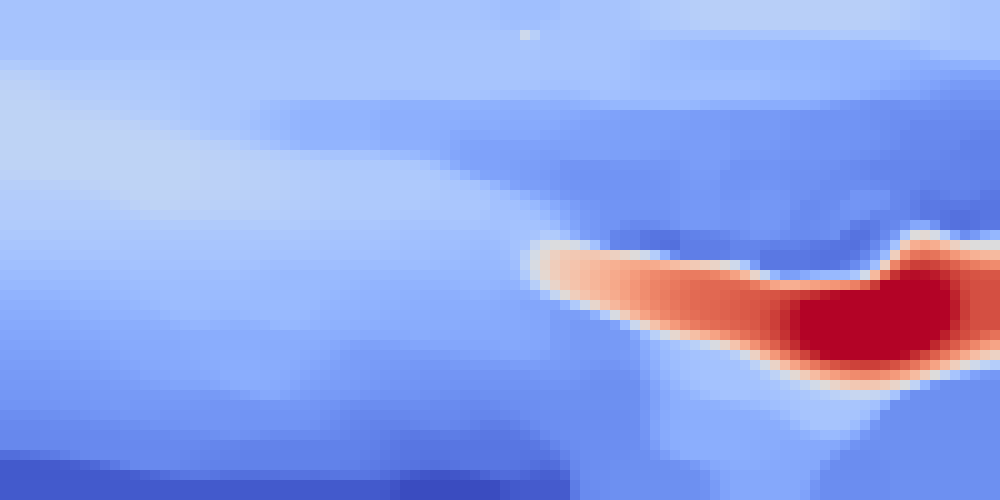
\includegraphics[width=40mm]{public/alpha_350}
            \vspace{-8mm}
            \caption*{Proposed Method, $\alpha$=350}
        \end{minipage} &
        \begin{minipage}[b]{40mm}
            \centering
            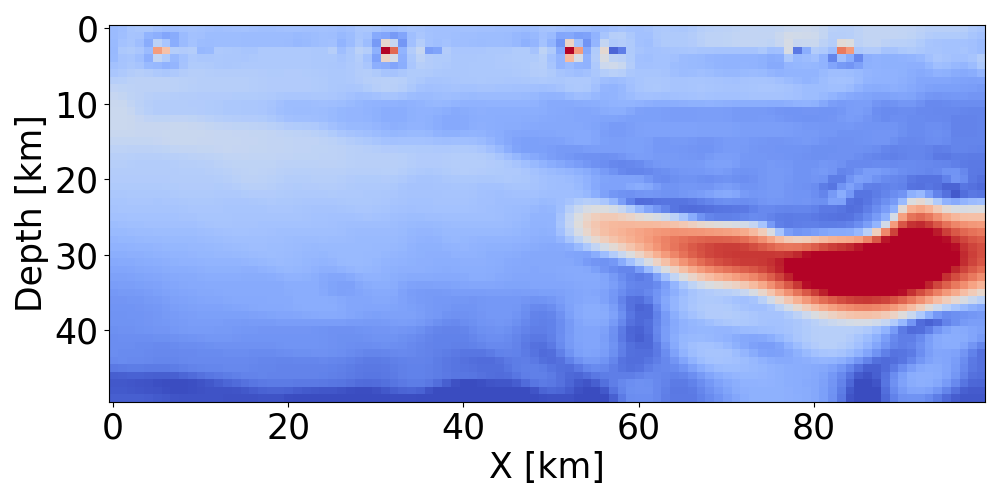
\includegraphics[width=40mm]{public/alpha_550}
            \vspace{-8mm}
            \caption*{Proposed Method, $\alpha$=550}
        \end{minipage} &
    \end{tabular}
    \vspace{-3mm}
    \caption{Velocity models and their corresponding reconstructions.}
    \label{fig:velocity-models}
\vspace{-\baselineskip}
\vspace{2mm}
\end{figure*}

%\begin{figure*}[htbp]
%\vspace{-\baselineskip}
%    \centering
%    \begin{tabular}{m{68mm} m{68mm} m{10mm}}
%        \begin{minipage}[b]{65mm}
%            \centering
%            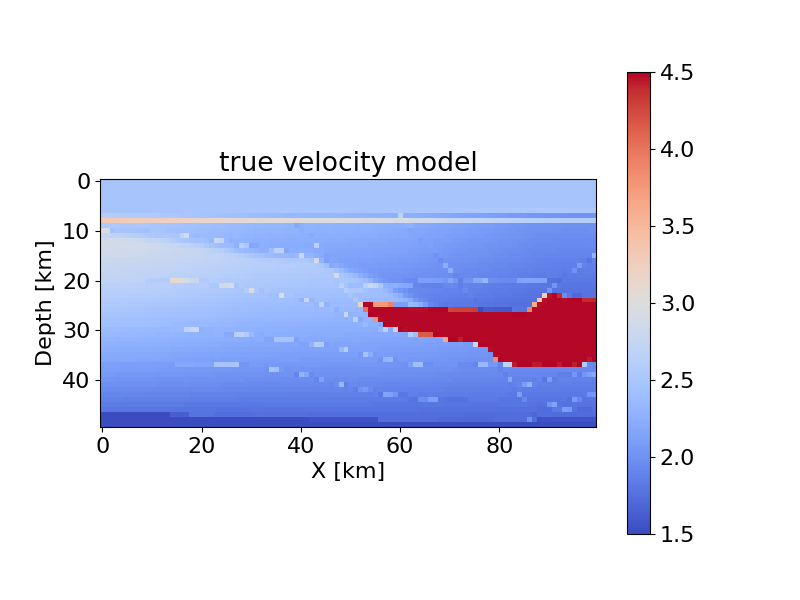
\includegraphics[width=65mm]{public/true}
%            \vspace{-7mm}
%            \caption*{\raisebox{2mm}{Background truth}}
%        \end{minipage} &
%        \begin{minipage}[b]{65mm}
%            \centering
%            
\includegraphics[width=65mm]{public/initial}
%            \vspace{-7mm}
%            \caption*{\raisebox{2mm}{Initial model}}
%        \end{minipage} &
%        \multirow[t]{3}{*}{\raisebox{-87mm}{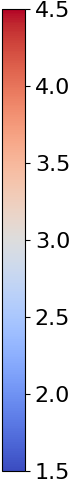
\includegraphics[height=70mm]{public/color-bar}}} \\
%
%        \begin{minipage}[b]{65mm}
%            \centering
%            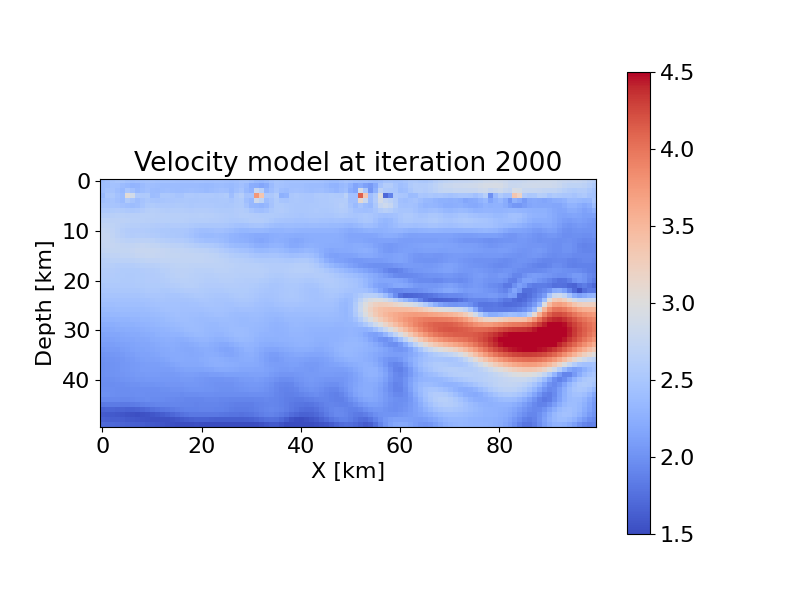
\includegraphics[width=65mm]{public/gradient}
%            \vspace{-7mm}
%            \caption*{\raisebox{2mm}{Standard FWI}}
%        \end{minipage} &
%        \begin{minipage}[b]{65mm}
%            \centering
%            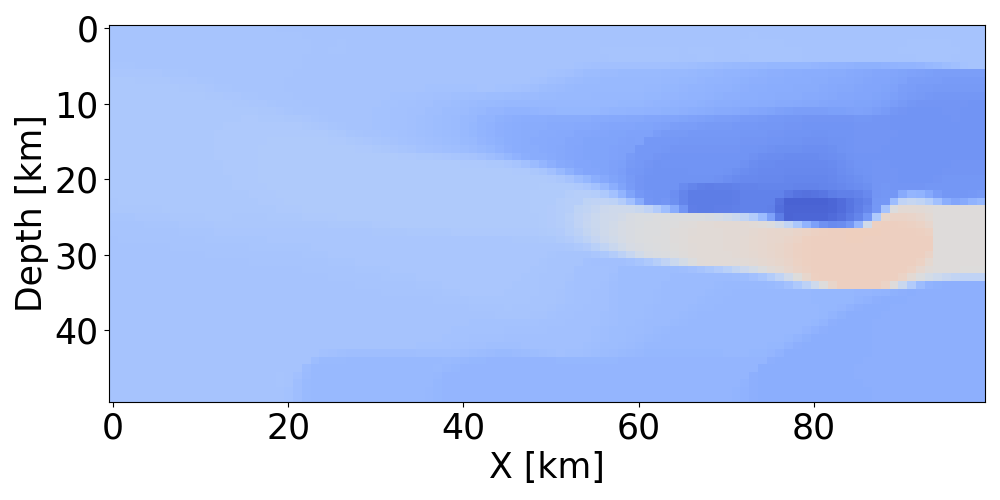
\includegraphics[width=65mm]{public/alpha_150}
%            \vspace{-7mm}
%            \caption*{Proposed Method, $\alpha = 150$}
%        \end{minipage} \\
%
%        \begin{minipage}[b]{65mm}
%            \centering
%            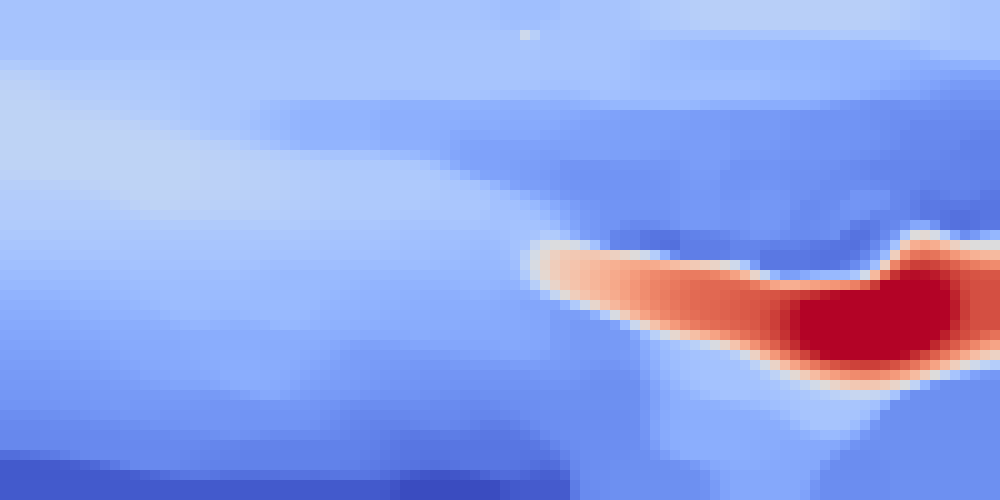
\includegraphics[width=65mm]{public/alpha_350}
%            \vspace{-7mm}
%            \caption*{Proposed Method, $\alpha = 350$}
%        \end{minipage} &
%        \begin{minipage}[b]{65mm}
%            \centering
%            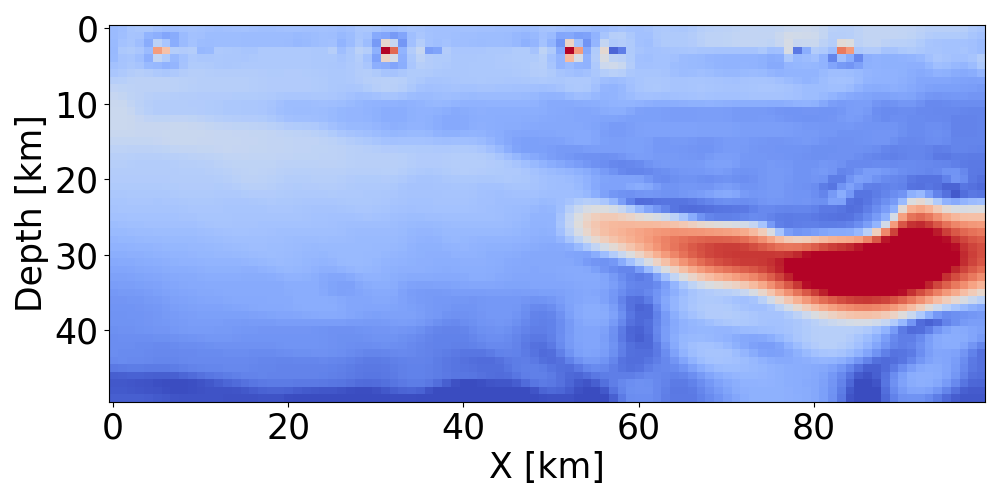
\includegraphics[width=65mm]{public/alpha_550}
%            \vspace{-7mm}
%            \caption*{Proposed Method, $\alpha = 550$}
%        \end{minipage} &
%    \end{tabular}
%    \caption{Velocity models and their corresponding reconstructions.}
%    \label{fig:velocity-models}
%\vspace{-\baselineskip}
%\end{figure*}

\begin{figure*}[htbp]
%\vspace{-\baselineskip}
    \centering
    \begin{minipage}{70mm}
        \centering
        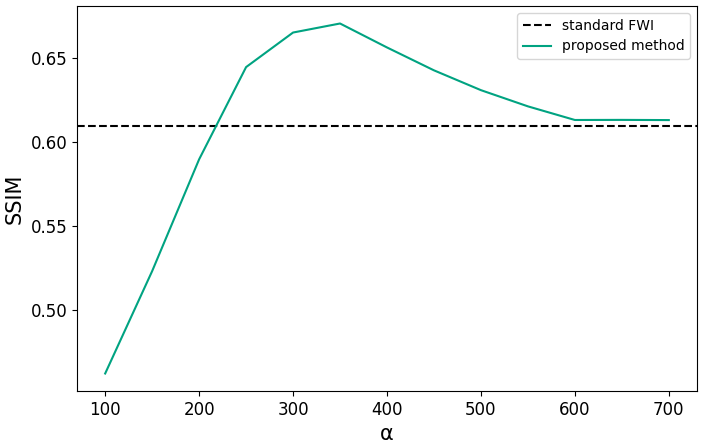
\includegraphics[width=\linewidth]{public/alpha-ssim}
        \vspace{-8mm}
        \caption{SSIM against the parameter of alpha.}
        \label{fig:alpha-ssim}
    \end{minipage}
    \hspace{10mm}
    \begin{minipage}{70mm}  % minipageで横並びに
        \centering
        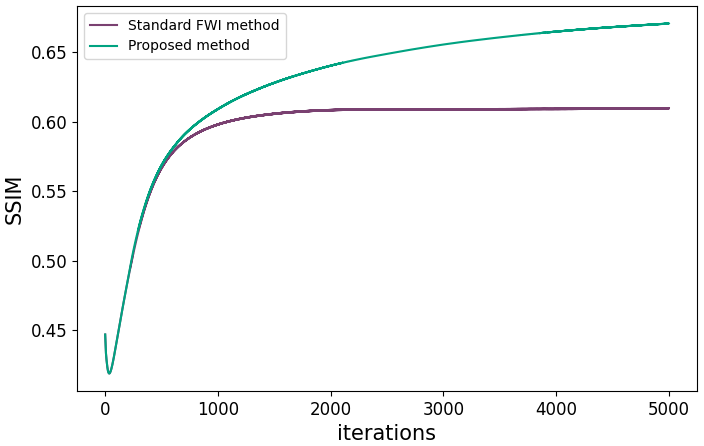
\includegraphics[width=\linewidth]{public/iters-ssim}
        \vspace{-8mm}
        \caption{SSIM against the number of iterations.}
        \label{fig:iters-ssim}
    \end{minipage}
\vspace{-\baselineskip}
\vspace{2mm}
\end{figure*}



\subsection{Experimental Setup}\label{subsec:experimental-setup}

To demonstrate the effectiveness of the TV and box constrained FWI, we conducted experiments where we compared with the standard FWI with gradient method~\eqref{eq:FWIWithGradient}, using the SEG/EAGE Salt and Overthrust Models.
The velocity model consists of 101 $\times$ 51 grid points.
The ground truth velocity model is generated by zooming and cropping Fig.\ref{fig:salt-model}, and the initial velocity model is generated by smoothing the ground truth velocity model with a Gaussian function with a standard deviation of 80.
The number of receivers and source shots are 101 and 20, respectively, and are placed on the surface at equal intervals.
The source waveform is a Ricker wavelet with a peak wavelet frequency of 10 Hz.
The gradient of $E$ is computed numerically using the Devito framework\cite{devito}.
The number of iterations is set to 5000.
In the standard FWI, the step size $\gamma$ is set to $1.0 \times 10^{-4}$.
In the TV and box constrained FWI, the step size $\gamma_1$ and $\gamma_2$ are set to $1.0 \times 10^{-4}$ and $1.0 \times 10^2$, respectively,
    and the lower and upper bounds of the velocity model $a$, $b$ are set to 1.5[km/s] and 4.5[km/s], respectively,
    and experiments are conducted with several $\alpha$ that is the upper bound of the $l_{1,2}$ norm.
%However, it should be noted that parameters such as $\alpha$, $a$, and $b$ were determined by referencing the ground truth data.
%In a practical application, this must be determined independently of this framework.


\subsection{Results and Discussion}\label{subsec:results-and-discussion}

Fig.\ref{fig:velocity-models} shows the ground truth, the initial model, and the reconstructed velocity models using the standard FWI and the TV and box constrained FWI with several $\alpha$.
When $\alpha$ is small, such as 150, the TV constraint is too strong, resulting in an excessively smooth model.
Conversely, when $\alpha$ is large, such as 550, the TV constraint is almost meaningless, and a model similar to the standard FWI is obtained.
When $\alpha$ is appropriate, such as 350, the TV constraint successfully eliminates wave-like artifacts and noise that appear at the source positions, resulting in a more accurate velocity model reconstruction.

%\begin{figure}[htbp]
%%\vspace{-\baselineskip}
%    \begin{center}
%        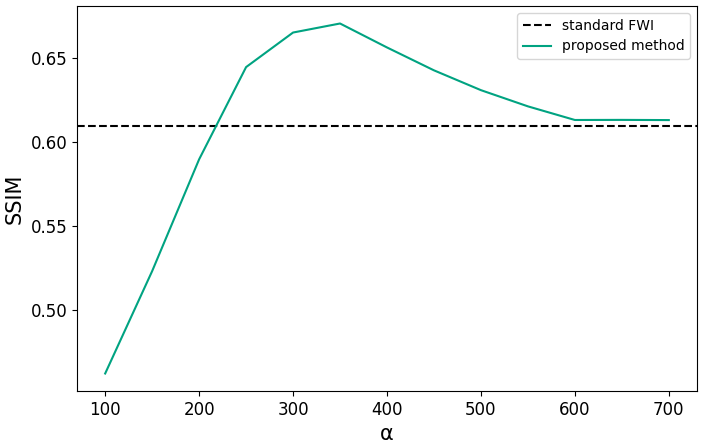
\includegraphics[width=80mm]{public/alpha-ssim}
%        \vspace{-5mm}
%        \caption{final SSIM against the number of iterations.}
%        \label{fig:alpha-ssim}
%    \end{center}
%    \vspace{-\baselineskip}
%\end{figure}

In Fig.\ref{fig:alpha-ssim}, we plot the Structural Similarity Index Measure (SSIM) against the parameter $\alpha$.
As mentioned earlier, the graph shows that when the value of $\alpha$ is small, the final SSIM decreases, and when the value of $\alpha$ is too large, the results become almost the same as the standard FWI, but not worse.
However, with an appropriately chosen $\alpha$, the graph shows that high SSIM values can be achieved.

%\begin{figure}[htbp]
%%\vspace{-\baselineskip}
%    \begin{center}
%        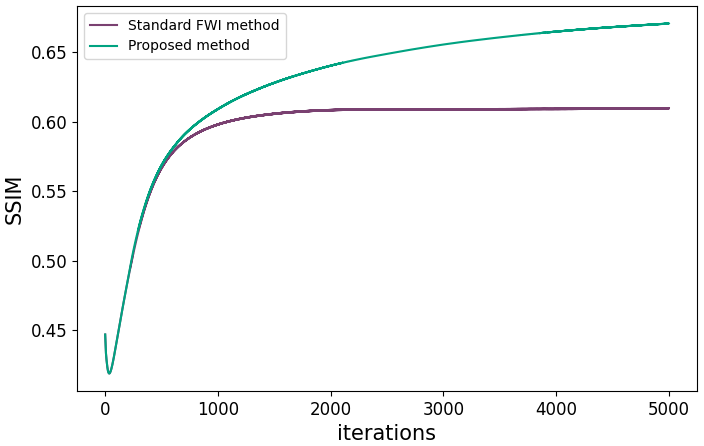
\includegraphics[width=80mm]{public/iters-ssim}
%        \vspace{-5mm}
%        \caption{SSIM against the number of iterations.}
%        \label{fig:iters-ssim}
%    \end{center}
%    \vspace{-\baselineskip}
%\end{figure}

In Fig.\ref{fig:iters-ssim}, we plot the SSIM against the number of iterations for both methods with $\alpha=350$.
With appropriate parameters, the proposed method consistently achieves higher SSIM values than the standard FWI at every iteration, indicating improved reconstruction accuracy.

